\section{Usecases}
\subsection{Use case diagram for the whole system}
\begin{figure}[hbt]
    \centering
    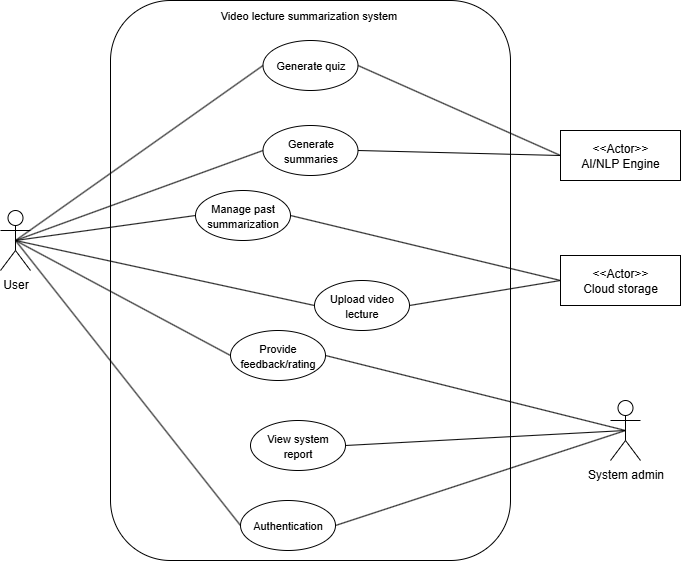
\includegraphics[width=1\linewidth]{system/images/whole_system.png}
    \caption{Use diagram for the whole system}
    \label{fig:p_ucsys}
\end{figure}

\subsection{Detail usecases}
\subsubsection{Use case: Upload a video}
\begin{table}[H]
    \begin{tabular}{|>{\raggedright\arraybackslash}p{0.25\textwidth}|>{\raggedright\arraybackslash}p{0.7\textwidth}|}
        \hline
        \multicolumn{1}{|>{\raggedright\arraybackslash}p{0.25\textwidth}|}{ID and Name} &
        \multicolumn{1}{>{\raggedright\arraybackslash}p{0.7\textwidth}|}{UC-01: Upload a video lecture} \\
        \hline
        Created by & Nguyen Binh Nguyen\\
        \hline
        Primary actor & User \\
        \hline
        Secondary actor & Secondary actor: System\\
        \hline
        Date created & 10/09/2024 \\
        \hline
        Description &
        The user uploads a video lecture file (or provides a video link) into the system. The system verifies the file format, size, and availability before storing it for transcription and further processing.\\
        \hline
        Trigger &
        A user selects the option to upload a new lecture video.\\
        \hline
        Preconditions &
        \begin{itemize}
            \item PRE-01: User's identity has been authenticated.
            \item PRE-02: The user has an active account in the system.
            \item PRE-03: The video file must be in a supported format (e.g., MP4, AVI, MKV) or a valid external link (e.g., YouTube).
        \end{itemize} \\
        \hline
        Postconditions &
        \begin{itemize}
            \item POST-01: The video is uploaded successfully and stored.
        \end{itemize} \\
        \hline
    \end{tabular}
\end{table}

\begin{table}[H]
    \begin{tabular}{|>{\raggedright\arraybackslash}p{0.25\textwidth}|>{\raggedright\arraybackslash}p{0.7\textwidth}|}
        \hline
        Postconditions &
        \begin{itemize}
            \item POST-02: The system queues the video for transcription.
            \item POST-3: The user is notified that the upload was successful.
        \end{itemize} \\
        \hline
        Normal flow &
        \begin{enumerate}
            \item NF-01: The user clicks on “Upload video.”
            \item NF-02: The system prompts for file upload or video link.
            \item NF-03: The user selects and submits the video.
            \item NF-04: The system validates the file/link and stores it.
            \item NF-05: The system notifies the user of successful upload.
        \end{enumerate} \\
        \hline
        Alternative flow &
        \begin{itemize}
            \item AF-01:  The user selects an unsupported video file
            \begin{enumerate}
                \item The system displays an error message indicating unsupported format.
                \item The user selects another video in a valid format.
                \item The Use Case continues from step 2.
            \end{enumerate}
        \end{itemize} \\
        \hline
    \end{tabular}
\end{table}

\subsubsection{Use case: Summarize a video}
\newpage


\begin{table}[H]
    \begin{tabular}{|>{\raggedright\arraybackslash}p{0.25\textwidth}|>{\raggedright\arraybackslash}p{0.7\textwidth}|}
        \hline
        \multicolumn{1}{|>{\raggedright\arraybackslash}p{0.25\textwidth}|}{ID and Name} &
        \multicolumn{1}{>{\raggedright\arraybackslash}p{0.7\textwidth}|}{UC-02: Summarize a video} \\
        \hline
        Created by & Nguyen Binh Nguyen\\
        \hline
        Primary actor & User \\
        \hline
        Secondary actor & Secondary actor: AI/NLP engine\\
        \hline
        Date created & 10/09/2024 \\
        \hline
        Description &
        The user requests the system to summarize the uploaded lecture. The system processes the transcript and generates a concise summary in bullet points, outline, or paragraph form.\\
        \hline
        Trigger &
        A user selects the option “Summarize Video” after transcript generation is complete.\\
        \hline
        Preconditions &
        \begin{itemize}
            \item PRE-01: User's identity has been authenticated.
            \item PRE-02: A video has already been uploaded and transcribed.
        \end{itemize} \\
        \hline
        Postconditions &
        \begin{itemize}
            \item POST-01: A summary is generated and displayed to the user.
            \item POST-02: The summary is stored for future reference.
        \end{itemize} \\
        \hline
        Normal flow &
        \begin{enumerate}
            \item NF-01: The user selects the “Summarize Video” option.
            \item NF-02: The system retrieves the transcript.
            \item NF-03: The system generates a summary.
        \end{enumerate} \\
        \hline
    \end{tabular}
\end{table}

\begin{table}[H]
    \begin{tabular}{|>{\raggedright\arraybackslash}p{0.25\textwidth}|>{\raggedright\arraybackslash}p{0.7\textwidth}|}
        \hline
        Normal flow &
        \begin{enumerate}
            \setcounter{enumi}{3}
            \item NF-04: The user views the summary.
        \end{enumerate} \\
        \hline
        Alternative flow &
        \begin{itemize}
            \item AF-01:  The user selects a summary style (bullet points, outline, paragraph).
            \begin{enumerate}
                \item The system generates the summary accordingly.
            \end{enumerate}
        \end{itemize} \\
        \hline
        Exception &
        \begin{itemize}
            \item The system detects no transcript exists.
            \begin{enumerate}
                \item The system notifies the user to upload or wait for transcription.
            \end{enumerate}
        \end{itemize}\\
        \hline
    \end{tabular}
\end{table}\\

\subsubsection{Use case: Generate a quiz}
\newpage

\begin{table}[H]
    \begin{tabular}{|>{\raggedright\arraybackslash}p{0.25\textwidth}|>{\raggedright\arraybackslash}p{0.7\textwidth}|}
        \hline
        \multicolumn{1}{|>{\raggedright\arraybackslash}p{0.25\textwidth}|}{ID and Name} &
        \multicolumn{1}{>{\raggedright\arraybackslash}p{0.7\textwidth}|}{UC-03: Generate a quiz} \\
        \hline
        Created by & Nguyen Binh Nguyen\\
        \hline
        Primary actor & User \\
        \hline
        Secondary actor & Secondary actor: AI/NLP engine\\
        \hline
        Date created & 10/09/2024 \\
        \hline
        Description &
        The user requests the system to generate a quiz from the transcript. The system analyzes key concepts and creates a set of questions with answers.\\
        \hline
        Trigger &
        A user selects the option “Generate Quiz.”\\
        \hline
        Preconditions &
        \begin{itemize}
            \item PRE-01: User's identity has been authenticated.
            \item PRE-02: A transcript or summary is available.
        \end{itemize} \\
        \hline
        Postconditions &
        \begin{itemize}
            \item POST-01: A quiz is generated and shown to the user.
            \item POST-02: The quiz is stored for practice or download.
        \end{itemize} \\
        \hline
        Normal flow &
        \begin{enumerate}
            \item NF-01: The user selects “Generate Quiz.”
            \item NF-02: The system analyzes the transcript.
            \item NF-03: The system creates quiz questions.
            \item NF-04: The quiz is displayed to the user.
        \end{enumerate} \\
        \hline
    \end{tabular}
\end{table}

\begin{table}[H]
    \begin{tabular}{|>{\raggedright\arraybackslash}p{0.25\textwidth}|>{\raggedright\arraybackslash}p{0.7\textwidth}|}
        \hline
        Alternative flow &
        \begin{itemize}
            \item AF-01: Choose quiz difficulty/length
            \begin{enumerate}
                \item The user selects quiz difficulty or number of questions.
                \item The system adjusts quiz generation accordingly.
            \end{enumerate}
        \end{itemize} \\
        \hline
        Exception &
        \begin{itemize}
            \item The transcript is too short.
            \begin{enumerate}
                \item The system notifies the user and suggests uploading a longer video.
            \end{enumerate}
        \end{itemize}\\
        \hline
    \end{tabular}
\end{table}

\subsubsection{Use case: Take a quiz \& get feedback}
\newpage
\begin{table}[H]
    \begin{tabular}{|>{\raggedright\arraybackslash}p{0.25\textwidth}|>{\raggedright\arraybackslash}p{0.7\textwidth}|}
        \hline
        \multicolumn{1}{|>{\raggedright\arraybackslash}p{0.25\textwidth}|}{ID and Name} &
        \multicolumn{1}{>{\raggedright\arraybackslash}p{0.7\textwidth}|}{UC-04: Take a quiz \& get feedback} \\
        \hline
        Created by & Nguyen Binh Nguyen\\
        \hline
        Primary actor & User \\
        \hline
        Secondary actor & Secondary actor: System, AI/NLP engine\\
        \hline
        Date created & 10/09/2024 \\
        \hline
        Description &
       The user takes the generated quiz. The system provides immediate or final feedback with correct answers and explanations.\\
        \hline
        Trigger &
        The user selects “Start Quiz.”\\
        \hline
        Preconditions &
        \begin{itemize}
            \item PRE-01: User's identity has been authenticated.
            \item PRE-02: A quiz has been generated.
        \end{itemize} \\
        \hline
        Postconditions &
        \begin{itemize}
            \item POST-01: User completes the quiz.
            \item POST-02: Results and feedback are displayed.
            \item POST-03: Performance is stored.
        \end{itemize} \\
        \hline
        Normal flow &
        \begin{enumerate}
            \item NF-01: The user selects “Start Quiz.”
            \item NF-02: The system presents questions.
            \item NF-03: The user submits answers.
            \item NF-04: The system evaluates answers.
            \item NF-05: Feedback is shown.
        \end{enumerate} \\
        \hline
    \end{tabular}
\end{table}

\begin{table}[H]
    \begin{tabular}{|>{\raggedright\arraybackslash}p{0.25\textwidth}|>{\raggedright\arraybackslash}p{0.7\textwidth}|}
        \hline
        Alternative flow &
        \begin{itemize}
            \item AF-01: User requests instant feedback
            \begin{enumerate}
                \item The system shows feedback after each question instead of at the end.
            \end{enumerate}
        \end{itemize} \\
        \hline
        Exception &
        \begin{itemize}
            \item Quiz session interrupted
            \begin{enumerate}
                \item The system saves progress, allowing resuming later.
            \end{enumerate}
        \end{itemize}\\
        \hline
    \end{tabular}
\end{table}

\subsubsection{Use case: Download/Export results}
\newpage 

\begin{table}[H]
    \begin{tabular}{|>{\raggedright\arraybackslash}p{0.25\textwidth}|>{\raggedright\arraybackslash}p{0.7\textwidth}|}
        \hline
        \multicolumn{1}{|>{\raggedright\arraybackslash}p{0.25\textwidth}|}{ID and Name} &
        \multicolumn{1}{>{\raggedright\arraybackslash}p{0.7\textwidth}|}{UC-05 Download/Export results} \\
        \hline
        Created by & Nguyen Binh Nguyen\\
        \hline
        Primary actor & User \\
        \hline
        Secondary actor & Secondary actor: System\\
        \hline
        Date created & 10/09/2024 \\
        \hline
        Description &
       The user downloads the generated summary, quiz, or results in a chosen format (PDF, Word, etc.).\\
        \hline
        Trigger &
        The user selects “Download” or “Export.”\\
        \hline
        Preconditions &
        \begin{itemize}
            \item PRE-01: User's identity has been authenticated.
            \item PRE-02: At least one summary or quiz result exists.
        \end{itemize} \\
        \hline
        Postconditions &
        \begin{itemize}
            \item POST-01: File is generated and made available.
            \item POST-02: File may be stored in user’s account history.
        \end{itemize} \\
        \hline
        Normal flow &
        \begin{enumerate}
            \item NF-01: User clicks “Download.”
            \item NF-02: System asks for format selection (PDF, DOCX, TXT).
            \item NF-03: User confirms.
            \item NF-04: The system generates files.
            \item NF-05: The user downloads the file.
        \end{enumerate} \\
        \hline
    \end{tabular}
\end{table}

\begin{table}[H]
    \begin{tabular}{|>{\raggedright\arraybackslash}p{0.25\textwidth}|>{\raggedright\arraybackslash}p{0.7\textwidth}|}
        \hline
        Alternative flow &
        \begin{itemize}
            \item AF-01: Share instead of download
            \begin{enumerate}
                \item The user selects “Share Link.”
                \item The system generates a shareable link.
            \end{enumerate}
        \end{itemize} \\
        \hline
        Exception &
        \begin{itemize}
            \item Export failure
            \begin{enumerate}
                \item The system shows an error and suggests retrying.
            \end{enumerate}
        \end{itemize}\\
        \hline
    \end{tabular}
\end{table}